%%%%%%%%%%%%%%%%%%%%%%%%%%%%%%%%%%%%%%%%%%%%%%%%%%%%%%%%%%%%%%%%%%%%%%%%%%%%%%%%%%%%%%%%%%%%%%%%%%%
%%%%%%%%%%%%%%%%%%%%%%%%%%%%%%%%%%%%%%%%%%%%%%%%%%%%%%%%%%%%%%%%%%%%%%%%%%%%%%%%%%%%%%%%%%%%%%%%%%%
%%%%%%%%%%%%%%%%%%%%%%%%%%%%%%%%%%%%%%%%%%%%%%%%%%%%%%%%%%%%%%%%%%%%%%%%%%%%%%%%%%%%%%%%%%%%%%%%%%%
%%%%%%%%%%%%%%%%%%%%%%%%%%%%%%%%%%%%%%%%%%%%%%%%%%%%%%%%%%%%%%%%%%%%%%%%%%%%%%%%%%%%%%%%%%%%%%%%%%%

\chapter{Metodología}

El presente trabajo resulta de una colaboración con el departamento de Gerontología, dependiente 
del Instituto de Ciencias de la Salud (ICSA); parte de esta colaboración incluye el acceso a los 
registros de PSG obtenidos por Vázquez Tagle y colaboradores \cite{VazquezTagle16}. 
A continuación se cita la metodología de aquél estudio de la manera más fiel posible.
%Así mismo se describe, a nivel de implementación, el análisis central de este trabajo: la prueba 
%de Priesltey-Subba Rao. 

\section{Participantes}

Los sujetos fueron elegidos usando un muestreo \textit{no probabilístico por 
conveniencia}\footnote{Esto implica que los resultados pueden  no ser interpolables a poblaciones 
más grandes} bajo los siguientes criterios de inclusión:
\begin{itemize}
\item Edad entre 60 y 85 años
\item Diestros (mano derecha dominante)
\item Sin ansiedad, depresión ni síndromes focales
\item No usar medicamentos o sustancias para dormir
\item Firma de consentimiento informado
\item Voluntario para el registro de PSG
\end{itemize}

Un total de 9 participantes cumplieron todos los criterios de inclusión y procedieron al registro 
de PSG; adicionalmente se tomaron registros de otros tres adultos mayores, bajo el consentimiento 
de éstos y de los responsables del proyecto (ver más adelante).
%
Todos los participantes fueron sometidos a una batería de pruebas neuropsicológicas para determinar
su estado cognoscitivo general (Neuropsi, MMSE), así como descartar cuadros depresivos (GDS, SATS) 
y cambios en la vida cotidiana (KATZ).
Usando los resultados obtenidos, los sujetos se dividieron en tres grupos:

\begin{table}[h]
\centering
\begin{tabular}{lcl}
\toprule
Grupo & Sujetos & Características \\
\midrule
Mn & 4 & Posible Deterioro Cognitivo \\
Nn & 5 & Sin PDC \\
ex & 3 & No satisfacen los criterios de inclusión \\
\bottomrule
\end{tabular}
\end{table}
%
%\begin{description}
%\item[Mn] (4 sujetos) Posible Deterioro Cognitivo
%\item[Nn] (5 sujetos) Sin PDC
%\item[ex] (3 sujetos) No satisfacen los criterios de inclusión
%\end{description}

El grupo ex se conforma de sujeto que incumplen al menos uno de los criterios de inclusión: {FGH} 
padece parálisis facial y posiblemente daño cerebral (síndromes focales), MGG padece depresión, 
EMT no califica como adulto mayor por su edad.
Se efectuaron todos los análisis sobre este grupo, con la finalidad de exhibir las capacidades y
limitaciones de las técnicas utilizadas; por ello este grupo es ignorado en la sección de 
resultados pero no en la discusión.

\begin{table}
\centering
\bordes{1.1}
\begin{tabular}{c}
\textbf{Datos generales de los participantes}
\vspace{1em}
\end{tabular}
{\small
\begin{tabular}{llcrrrrrrr}
\toprule
 \phantom{.}&
 & {Sexo} & {Edad} & {Escol.} & {Neuropsi} & {MMSE} & {SATS} & {KATZ} & {Gds} \\
\midrule
\multicolumn{6}{l}{{Grupo Nn}}\\
&VCR    & F    & 59\pz & 12\pz & 107\pz & 29\pz & 21\pz & 0\pz & 3\pz \\
&MJH    & F    & 72\pz & 9\pz  & 113\pz & 30\pz & 18\pz & 0\pz & 0\pz \\
&JAE    & F    & 78\pz & 5\pz  & 102\pz & 28\pz & 19\pz & 0\pz & 5\pz \\
&GHA    & M    & 65\pz & 9\pz  & 107.5  & 30\pz & 23\pz & 0\pz & 7\pz \\
&MFGR   & F    & 67\pz & 11\pz & 110\pz & 30\pz & 18\pz & 0\pz &      \\
\rowcolor{gris}
&\multicolumn{1}{c}{$\widehat{\mu}$} & 
               & 68.2  & 9.2   & 107.9  & 29.4  & 19.8  & 0.0  & 3.0  \\
\rowcolor{gris}
&\multicolumn{1}{c}{$\widehat{\sigma}$} & 
               & 7.2   & 2.7   & 4.1    & 0.9   & 2.2   & 0.0  & 3.0  \\
\midrulec
%\hline
\multicolumn{6}{l}{{Grupo Mn}}\\
&CLO    & F    & 68\pz & 5\pz  & 81\pz & 28\pz & 22\pz & 1\pz & 6\pz \\
&RLO    & F    & 63\pz & 9\pz  & 90\pz & 29\pz & 20\pz & 0\pz & 3\pz \\
&RRU    & M    & 69\pz & 9\pz  & 85\pz & 27\pz & 10\pz & 0\pz & 3\pz \\
&JGZ    & M    & 65\pz & 11\pz & 87\pz & 25\pz & 20\pz & 0\pz & 1\pz \\
\rowcolor{gris}
&\multicolumn{1}{c}{$\widehat{\mu}$} & 
              & 66.3   & 8.5   & 85.8  & 27.3  & 18.0  & 0.3  & 3.3  \\
\rowcolor{gris}
&\multicolumn{1}{c}{$\widehat{\sigma}$} & 
              & 2.8    & 2.5   & 3.8   & 1.7   & 5.4   & 0.5  & 2.1  \\
\midrulec
%\hline
\multicolumn{6}{l}{{Grupo ex}}\\
&FGH    & M    & 71\pz   & 9\pz    & 83.5     & 21\pz   & 23\pz   & 0\pz    & 4\pz  \\
&MGG    & F    & 61\pz   & 9\pz    & 114\pz      & 28\pz   & 29\pz   & 1\pz    & 14\pz \\
&EMT    & M    & 50\pz   & 22\pz   & 106\pz      & 30\pz   & 15\pz   & 0\pz    & 4\pz  \\
\bottomrule
\end{tabular} 
}
\label{tab_sujetos}
\caption{Resultados de las pruebas neuropsicológicas 
}
\end{table}

%%%%%%%%%%%%%%%%%%%%%%%%%%%%%%%%%%%%%%%%%%%%%%%%%%%%%%%%%%%%%%%%%%%%%%%%%%%%%%%%%%%%%%%%%%%%%%%%%%%
%%%%%%%%%%%%%%%%%%%%%%%%%%%%%%%%%%%%%%%%%%%%%%%%%%%%%%%%%%%%%%%%%%%%%%%%%%%%%%%%%%%%%%%%%%%%%%%%%%%

\section{Registro del polisomnograma}

Los adultos mayores participantes fueron invitados a acudir a las instalaciones de la Clínica 
Gerontológica de Sueño (ubicadas dentro del Instituto de Ciencias de la Salud) para llevar a cabo 
el registro. Los participantes recibieron instrucciones de realizar una rutina normal de 
actividades durante la semana que precedió al estudio, y se les recomendó que no ingirieran bebidas 
alcohólicas o energizantes (como café o refresco) durante las 24 horas previas al experimento, ni 
durmieran siesta ese día.

El protocolo de PSG incluye 19 electrodos de EEG, 4 electrodos de EOG para registrar movimientos 
oculares horizontales y verticales, y 2 electrodos de EMG colocados en los músculos submentonianos 
para registrar la actividad muscular. 
La colocación de los electrodos para registrar la actividad EEG se realizó siguiendo las 
coordenadas del Sistema Internacional 10--20.

Las señales fueron amplificadas (amplificador de alta ganancia en cadena), filtradas (filtro paso 
de banda de 0.5--30 Hz) y digitalizadas para su posterior análisis.
En la tabla \ref{frecuencias} se reportan la duración de estos registros para cada sujeto.

Debido a problemas técnicos el registro se efectúo a 512 puntos por segundo (Hz) para algunos
participantes, y a 200 Hz para otros; en ambos casos se satisface la recomendación de la AASM de un 
mínimo de 128 Hz. 

La clasificación del PSG en fases de sueño se realizó \textit{manualmente} sobre épocas de 30 
segundos siguiendo los criterios estandarizados de la AAMS \cite{Hori01}.

%Debido a un cambio en el polisomnógrafo 
%usado, la frecuencia de muestreo (en Hz) cambia entre sujetos.

\begin{table}
\centering
\bordes{1.2}
\begin{tabular}{c}
\textbf{Datos generales sobre los registros de PSG}
\vspace{1em}
\end{tabular}
{\small
\begin{tabular}{llcrrcrrr}
\toprule
    \phantom{.}&
    &\multirow{2}{*}{\bordes{1}\begin{tabular}{l}Frecuencia\\ muestreo\end{tabular}}
    \bordes{1.2}
    & \multicolumn{2}{c}{Total} & \phantom{l}   & \multicolumn{3}{c}{MOR*}\\
    \cmidrule{4-5}  \cmidrule{7-9}
    &&          &Puntos  &  Tiempo   &&Puntos  &  Tiempo   &  \% MOR \\
\midrule
\multicolumn{6}{l}{{Grupo Nn}}\\
&VCR &200       & 5166000&   7:10:30 &&438000  &   0:36:30 & 8.5\% \\
&MJH &512       &15851520&   8:36:00 &&1950720 &   1:03:30 &12.3\% \\
&JAE &512       &13931520&   7:33:30 &&2626560 &   1:25:30 &18.9\% \\
&GHA &200       &6558000 &   9:06:00 &&330000  &   0:27:30 & 5.0\% \\
&MFGR&200       &4932000 &   6:51:00 &&570000  &   0:47:30 &11.6\% \\

\rowcolor{gris}
&\multicolumn{1}{c}{$\widehat{\mu}$}  
              & &        & 7:51:30   &&        &   0:52:06 &11.2\% \\
\rowcolor{gris}
&\multicolumn{1}{c}{$\widehat{\sigma}$} 
              & &        & 0:57:36   &&        &   0:23:00 & 5.1\% \\
\midrulec

\multicolumn{6}{l}{{Grupo Mn}}\\
&CLO &512       &14499840&   7:52:00 &&2027520 &   1:06:00 &14.0\% \\
&RLO &512       &12994560&   7:03:00 &&1520640 &   0:49:30 &11.7\% \\
&RRU &200       &2484000 &   3:27:00 &&228000  &   0:19:00 & 9.2\% \\
&JGZ &512       &18539520&  10:03:30 &&506880  &   0:16:30 & 2.7\% \\

\rowcolor{gris}
&\multicolumn{1}{c}{$\widehat{\mu}$}  
              & &        & 7:06:23   &&        &   0:37:45 &9.4\% \\
\rowcolor{gris}
&\multicolumn{1}{c}{$\widehat{\sigma}$} 
              & &        & 2:44:55   &&        &   0:24:05 &4.9\% \\
\midrulec

\multicolumn{6}{l}{{Grupo ex}}\\
&FGH &512       &6220800 &   3:22:30 &&337920  &   0:11:00 & 5.4\% \\
&MGG &512       &15820800&   8:35:00 &&2549760 &   1:23:00 &16.1\% \\
&EMT &512       &21857280&  11:51:30 &&721920  &   0:23:30 & 3.3\% \\
\bottomrule
\end{tabular}
}
\caption{Cantidad de datos registrados para cada sujeto. *Dado que el sueño MOR aparece fragmentado,
se reporta la suma de tales tiempos.}
\label{frecuencias}
\end{table}

%%%%%%%%%%%%%%%%%%%%%%%%%%%%%%%%%%%%%%%%%%%%%%%%%%%%%%%%%%%%%%%%%%%%%%%%%%%%%%%%%%%%%%%%%%%%%%%%%%%
%%%%%%%%%%%%%%%%%%%%%%%%%%%%%%%%%%%%%%%%%%%%%%%%%%%%%%%%%%%%%%%%%%%%%%%%%%%%%%%%%%%%%%%%%%%%%%%%%%%

\section{Aplicación de la prueba PSR}

Los registros digitalizados de PSG fueron convertidos a formato de texto bajo la codificación 
ASCII, a razón de un archivo por cada canal. 
Las épocas MOR, clasificadas manualmente, fueron indicadas en archivos a parte.

Como se mencionó en secciones anteriores, la prueba PSR está pensada para series de tiempo con 
media 0, varianza finita y espectro puramente continuo. Se espera que la segunda condición se 
cumpla para los registros de PSG; las otras dos condiciones fueron \textit{forzadas}, sustrayendo 
la media y la componente periódica (estimadas) del proceso.
Para lo anterior, se usó el algoritmo no-paramétrico STL (Seasonal-Trend decomposition using 
Loess) \cite{Cleveland1990} y que está implementado en R bajo la función \texttt{stl()}.

%La prueba PSR se encuentra implementado en R bajo la función \texttt{stationarity()} del paquete 
%\texttt{fractal}.
%Los resultados de la prueba PSR, aplicado a todas las épocas contenidas en los registros de PSG,
%fueron almacenados para su análisis posterior.

El registro de PSG por cada canal fueron analizados por separado, y éstos a su vez fueron divididos
en épocas de 30 segundos de duración (variando el número de puntos según la frecuencia de muestreo);
cada época fue clasificada como \textit{estacionaria} si, no pudo rechazarse la hipótesis de 
estacionariedad usando la prueba PSR ($p < 0.05$).
La cantidad de épocas estacionarias para cada individuo, durante sueño MOR y NMOR, se muestra en 
las tablas \ref{total_gpos_total} y \ref{total_gpos_mor}; debido a la gran variabilidad entre los 
sujetos para la duración del sueño MOR, para el análisis no se consideró el total de épocas sino la 
proporción de éstas en cada etapa de sueño. 

\begin{figure}
\centering
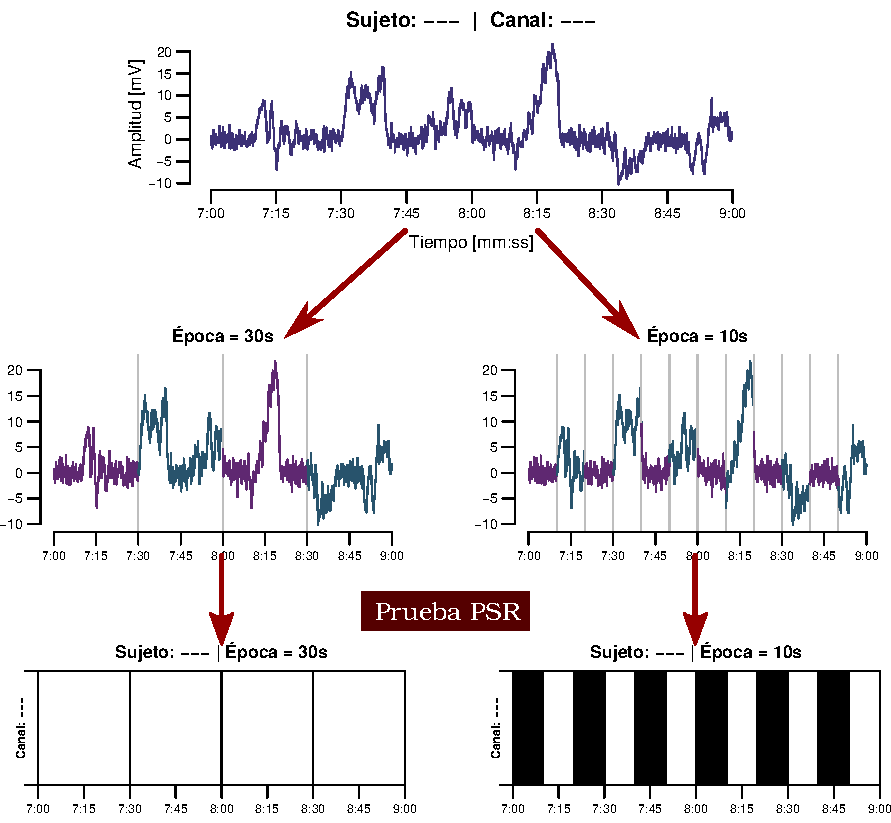
\includegraphics[width=\linewidth]{./img_diagramas/epocas_diferentes_v2.pdf}
\caption{Esquema de cómo se tomaron diferentes tamaños de época para estudiar los registros de 
PSG}
\label{epocas_diferentes}
\end{figure}



%%%%%%%%%%%%%%%%%%%%%%%%%%%%%%%%%%%%%%%%%%%%%%%%%%%%%%%%%%%%%%%%%%%%%%%%%%%%%%%%%%%%%%%%%%%%%%%%%%%
%%%%%%%%%%%%%%%%%%%%%%%%%%%%%%%%%%%%%%%%%%%%%%%%%%%%%%%%%%%%%%%%%%%%%%%%%%%%%%%%%%%%%%%%%%%%%%%%%%%
%%%%%%%%%%%%%%%%%%%%%%%%%%%%%%%%%%%%%%%%%%%%%%%%%%%%%%%%%%%%%%%%%%%%%%%%%%%%%%%%%%%%%%%%%%%%%%%%%%%
%%%%%%%%%%%%%%%%%%%%%%%%%%%%%%%%%%%%%%%%%%%%%%%%%%%%%%%%%%%%%%%%%%%%%%%%%%%%%%%%%%%%%%%%%%%%%%%%%%%